% Luonnolliset luvut esitellään nyt kokonaislukujen alussa.

% engl. \emph{natural numbers, counting numbers} ruots. \emph{naturliga tal}
% 
% 
% \laatikko{Luonnollisia lukuja käytetään kolmeen eri tarkoitukseen:
% 
% \begin{enumerate}
% \item Lukumäärien ilmoittamiseen (kardinaaliluvut)
% \item Järjestyksen ilmoittamiseen (ordinaaliluvut)
% \item Indeksointiin ja asioiden nimeämiseen
% \end{enumerate}
% }


% \subsection*{Tehtäviä}
% 
% \begin{tehtava}
% 
% Onko kardinaali vai ordinaali vai indeksointi?
% 
% \end{tehtava}

\section*{Kokonaisluvut}

Yksinkertaisimmat käyttämämme luvut ovat lukumäärien ilmaisemiseen käytetyt $0, 1, 2, 3, \ldots$. Näitä kutsutaan \emph{luonnollisiksi luvuiksi}, ja niiden joukkoa eli kaikkia luonnollisia lukuja yhdessä merkitään symbolilla $\mathbb{N}$.
Nolla määritellään tässä luonnolliseksi luvuksi, mutta tästä ei ole yhteistä sopimusta: eräät pitävät nollaa luonnollisena lukuna ja toiset eivät.

Luonnollisille luvuille $m$ ja $n$ on määritelty yhteenlasku $m + n$, esimerkiksi $5 + 3 = 8$.

Luonnollisten lukujen $m$ ja $n$ kertolasku määritellään peräkkäisinä yhteenlaskuina
\laatikko{
\[m \cdot n = \underbrace{m + m + \ldots + m}_{n\text{ kpl}} = \underbrace{n + n + \ldots + n}_{m\text{ kpl}}.\]
}

Nollalla kertomisen ajatellaan olevan ''tyhjä yhteenlasku'' eli nolla:

\laatikko{
\[0 \cdot m = 0\]
}

Luonnollisten lukujen $m$ ja $n$ erotus määritellään yhteenlaskun avulla:
$m-n$ on luku $k$, jolle $k + n = m$. Kahden luonnollisen luvun erotus
ei kuitenkaan aina ole luonnollinen luku, esimerkkinä $3 - 5$.
Ratkaisemme ongelman määrittelemällä kullekin luonnolliselle
luvulle vastaluvun.

\laatikko{
Jokaisella luvulla $n$ on vastaluku $-n$, jolle pätee $n+(-n)=0$.
}

Luonnolliset luvut ja niiden vastaluvut muodostavat yhdessä
kokonaislukujen joukon
\[\mathbb{Z} = \{\ldots, -2, -1, 0, 1, 2, \ldots\}.\]
Kun käytämme kokonaislukuja, voidaan kahden luvun erotus määritellä
yhteenlaskun ja vastaluvun avulla yksinkertaisesti:

\laatikko{
\[m-n = m+(-n)\]
}

    Esimerkiksi luvun $2$ vastalukua merkitään $-2$, ja sille pätee $2+(-2)=0$. Vastaavasti luvun $-2$ vastaluku on sellainen luku, joka laskettuna yhteen luvun $-2$ kanssa antaa luvun $0$. Tämä on tietysti $2$, koska $-2+2=0$. Näin voidaan huomata, että $-(-2)=2$.
    


\subsection*{Yhteen- ja vähennyslasku}

    Kysymys: Mitä saadaan, kun luvusta $5$ vähennetään luku $-8$?
    
    Negatiivisten ja positiivisten lukujen yhteen- ja vähennyslaskut voidaan helposti tulkita lukusuoran avulla.
    
    % tässä on vähän kyseenalaista käyttää sekaisin sanallista ja numeerista esitystä
    
    $5+8$ ''viiteen lisätään kahdeksan''
    \begin{center}
      \begin{lukusuora}{-1}{14}{14}
        %\lukusuoranuolialas{5}{13}
        %\lukusuoranuolialas{0}{8}
        {\color{red} \lukusuoravaliss{0}{5}{$0$}{$5$}}
        \lukusuorauusi
        {\color{red} \lukusuoravaliss{8}{13}{$8$}{${\color{black}13}$}}
        {\color{blue} \lukusuoravaliss{0}{8}{$0$}{$8$}}
       \end{lukusuora}
       ${\color{red}5}+{\color{blue}8}=13$
    \end{center}
    
    $5+(+8)$ ''viiteen lisätään plus kahdeksan''
    
    $+8$ tarkoittaa samaa kuin $8$. '$+$'-merkkiä käytetään luvun edessä silloin, kun halutaan korostaa, että kyseessä on nimenomaan positiivinen luku.
    
%säädetään kuva vähän irti tuosta edeltävästä tektistä
%\vspace{0.3cm}     
    
    \begin{center}
          \begin{lukusuora}{-1}{14}{14}
        {\color{red} \lukusuoravaliss{0}{5}{$0$}{$5$}}
        \lukusuorauusi
        {\color{red} \lukusuoravaliss{8}{13}{$8$}{${\color{black}13}$}}
        {\color{blue} \lukusuoravaliss{0}{8}{$0$}{$8$}}
       \end{lukusuora}
       ${\color{red}5}+({\color{blue}+8})=13$
    \end{center}
    
    $5-(+8)$ ''viidestä vähennetään $+8$''
    
    Tämä tarkoittaa samaa kuin $5-8$. Lukusuoralla siis liikutaan 8 pykälää taaksepäin.

%säädetään kuva vähän irti tuosta edeltävästä tektistä
\vspace{0.3cm}     
    
    \begin{center}
              \begin{lukusuora}{-4}{8}{14}
        {\color{blue} \lukusuoravaliss{-3}{5}{\color{black}$-3$}{$5$}}
        \lukusuorauusi
%        {\color{red} \lukusuoravaliss{8}{13}{$8$}{${\color{black}13}$}}
        {\color{red} \lukusuoravaliss{0}{5}{$0$}{$5$}}
       \end{lukusuora}
       ${\color{red}5}-({\color{blue}+8})=-3$
    \end{center}


%lukiolaiset pitivät näitä epäselvinä kuvina
    
    Mitä tapahtuu, kun lisätään negatiivinen luku? Kun lukuun lisätään $1$, se kasvaa yhdellä. Kun lukuun lisätään $0$, se ei kasva lainkaan. Kun lukuun lisätään negatiivinen luku, esimerkiksi $-1$, on luonnollista ajatella, että se pienenee. Tällä logiikalla negatiivisen luvun lisäämisen pitäisi siis pienentää alkuperäistä lukua. Siksi on sovittu, että $5+(-8)$ on yhtä suuri kuin $5-8$.
    
%säädetään kuva vähän irti tuosta edeltävästä tektistä
\vspace{0.3cm}     

    \begin{center}
                 \begin{lukusuora}{-4}{8}{14}
        {\color{blue} \lukusuoravaliss{-3}{5}{\color{black}$-3$}{$5$}}
        \lukusuorauusi
%        {\color{red} \lukusuoravaliss{8}{13}{$8$}{${\color{black}13}$}}
        {\color{red} \lukusuoravaliss{0}{5}{$0$}{$5$}}
       \end{lukusuora}
       ${\color{red}5}+({\color{blue}-8})=-3$
    \end{center}
    
    
    $5-(-8)$ ''viidestä vähennetään miinus kahdeksan''
    
    Negatiivisen luvun lisääminen on vastakohta positiivisen luvun lisäämiselle. Tällöin on luonnollista, että negatiivisen luvun vähentäminen on vastakohta positiivisen luvun vähentämiselle. Koska positiivisen luvun vähentäminen pienentää lukua, pitäisi negatiivisen luvun vähentämisen kasvattaa lukua. Tämän vuoksi on sovittu, että $5-(-8)$ tarkoittaa samaa kuin $5+8$.
    
%säädetään kuva vähän irti tuosta edeltävästä tektistä
\vspace{0.3cm}     
        
    \begin{center}
    \begin{lukusuora}{-1}{14}{14}
        {\color{red} \lukusuoravaliss{0}{5}{$0$}{$5$}}
        \lukusuorauusi
        {\color{red} \lukusuoravaliss{8}{13}{$8$}{${\color{black}13}$}}
        {\color{blue} \lukusuoravaliss{0}{8}{$0$}{$8$}}
       \end{lukusuora}
       ${\color{red}5}-({\color{blue}-8})=13$
    \end{center}


\laatikko{
Yhteen- ja vähennyslaskun merkkisäännöt

\begin{itemize}
\item $a+(-b)=a-b=a-(+b)$
\item $-(-a)=a$
\item $a-(-b)=a+b=a+(+b)$
\end{itemize}
}

\laatikko{
Yhteen- ja vähennyslasku kumoavat toisensa

\begin{itemize}
\item $a+b-b=a$
\item $a-b+b=a$
\end{itemize}
}


\subsection*{Kertolasku}

    Samaan logiikkaan perustuen on sovittu myös merkkisäännöt positiivisten ja negatiivisten lukujen kertolaskuissa. Kun negatiivinen ja positiivinen luku kerrotaan keskenään, saadaan negatiivinen luku, mutta kun kaksi negatiivista lukua kerrotaan keskenään, saadaan positiivinen luku.

    $3 \cdot 4$ ''kolme kappaletta nelosia''
    
   \begin{center}
    \begin{lukusuora}{-1}{14}{14}
	\color{red} \lukusuoravaliss{0}{4}{$0$}{$4$}
	\color{red} \lukusuoravaliss{4}{8}{$4$}{$8$}
	\color{red} \lukusuoravaliss{8}{12}{$8$}{$12$}

      \end{lukusuora}
      $3\cdot {\color{red}4}=12$
    \end{center}
    
    $3 \cdot (-4)$ ''kolme kappaletta miinus-nelosia''
    
    
    \begin{center}
    \begin{lukusuora}{-13}{2}{14}
	\color{red} \lukusuoravaliss{-12}{-8}{$-12$}{$-8$}
	\color{red} \lukusuoravaliss{-8}{-4}{$-8$}{$-4$}
	\color{red} \lukusuoravaliss{-4}{0}{$-4$}{$0$}

      \end{lukusuora}
      $3\cdot ({\color{red}-4})=-12$
    \end{center}
    
    $-3 \cdot 4$ ''miinus-kolme nelinkertaistetaan''
    
    \begin{center}
    \begin{lukusuora}{-13}{2}{14}
	\color{red} \lukusuoravaliss{-12}{-9}{$-12$}{$-9$}
	\color{red} \lukusuoravaliss{-9}{-6}{$-9$}{$-6$}
	\color{red} \lukusuoravaliss{-6}{-3}{$-6$}{$-3$}
	\color{red} \lukusuoravaliss{-3}{0}{$-3$}{$0$}

      \end{lukusuora}
      ${\color{red}-3}\cdot 4=-12$
    \end{center}
    
    $-3 \cdot (-4)$ ''miinus-kolme miinus-nelinkertaistetaan''
    
    \begin{center}
    \begin{lukusuora}{-1}{14}{14}
	\color{red} \lukusuoravaliss{12}{9}{$12$}{$9$}
	\color{red} \lukusuoravaliss{9}{6}{$9$}{$6$}
	\color{red} \lukusuoravaliss{6}{3}{$6$}{$3$}
	\color{red} \lukusuoravaliss{3}{0}{$3$}{$0$}

      \end{lukusuora}
      ${\color{red}-3}\cdot (-4)=12$
    \end{center}

\subsection*{Jakolasku}

        Kun ensin kerrotaan jollain ja sitten jaetaan samalla luvulla, päädytään takaisin samaan, mistä lähdettiin.  Jakolaskujen merkkisäännöt on sovittu niin, että tämä ominaisuus säilyy. Ne ovat siis samat kuin kertolaskujen merkkisäännöt.
    
    Esimerkiksi haluamme, että $(-12):(-3)\cdot (-3)=-12$. Nyt voimme kysyä, mitä laskun $(-12):(-3)$ tulokseksi pitäisi tulla, jotta jakolasku ja kertolasku säilyvät toisilleen käänteisinä, eli mikä luku kerrottuna $-3$:lla on $-12$. Kertolaskun merkkisäännöistä nähdään helposti, että tämän luvun täytyy olla $+4$ eli $4$. Niinpä on sovittu, että $(-12):(-3)=12:3=4$.

\laatikko{
Kerto- ja jakolaskun merkkisäännöt
\begin{itemize}
\item $a\cdot (-b)=(-a)\cdot b=-(ab)$
\item $(-a)\cdot (-b)=a\cdot b=ab$
\item $(-a):b=a:(-b)=-\dfrac{a}{b}$
\item $(-a):(-b)=a: b=\dfrac{a}{b}$
\end{itemize}
}

\laatikko{
Kerto- ja jakolasku kumoavat toisensa
\begin{itemize}
\item $a\cdot b:b=a$
\item $a:b\cdot b=a$
\end{itemize}
}

    \subsection*{Jaollisuus ja tekijöihinjako}

   
    \laatikko{
    Kokonaisluku $a$ on jaollinen kokonaisluvulla $b$, jos on olemassa kokonaisluku $c$ niin, että $a = b \cdot c$. Tällöin sanotaan myös, että $b$ on $a$:n tekijä.
    }
    
    \begin{esimerkki}
    \begin{enumerate}[a)]
    \item Luku $-12$ on jaollinen luvulla $3$:lla, sillä $-12 = 3 \cdot (-4)$.
    \item $-12$ ei ole jaollinen $5$:llä, sillä ei ole kokonaislukua, joka kerrottuna viidellä olisi $12$.
    \end{enumerate}
    \end{esimerkki}
    
    

    
    Yllä jaollisuus määritellään kertolaskun avulla. Jaollisuuden voi määritellä myös jakolaskun avulla niin, että $a$ on jaollinen $b$:llä, mikäli $a:b$ on kokonaisluku. Esimerkiksi $12$ on jaollinen $3$:lla, koska $12:3 = 4$, joka on kokonaisluku.
    %Tämä määritelmä vaatii kuitenkin, että $b \neq 0$, joten sitä ei voida pitää yleispätevänä määritelmänä jaollisuudelle. Se on kuitenkin monesti yksinkertaisempi tapa ajatella.
   
    \begin{center}
     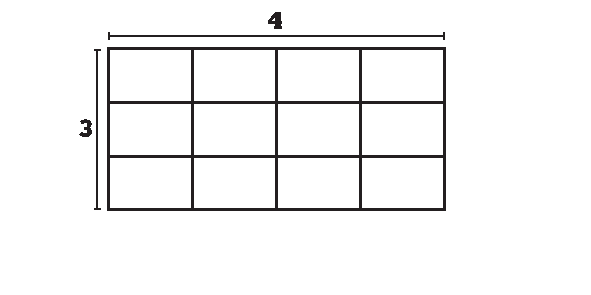
\includegraphics[scale=0.85]{pictures/Kuva2-4-3x4.pdf}
    \end{center}
    
    Kaikki luvut ovat jaollisia itsellään ja luvulla $1$. Esimerkiksi $7=7 \cdot 1=1 \cdot 7$, joten $7$ on jaollinen $1$:llä ja $7$:llä.
    
    \laatikko{
    \emph{Alkuluku} on ykköstä suurempi luku, joka on jaollinen ainoastaan luvulla $1$ ja itsellään.
    }
    
    Esimerkiksi luvut 2, 3, 5, 7, 11, 13, 17 ja 19 ovat alkulukuja.
    
    Kokonaisluvun $n$ tekijöitä, jotka ovat alkulukuja, kutsutaan alkutekijöiksi.
    
    \laatikko{
    \textbf{Aritmetiikan peruslause}
    
    Jokainen ykköstä suurempi kokonaisluku voidaan esittää yksikäsitteisesti alkulukujen tulona.
    }
    
   Aritmetiikan peruslause todistetaan kurssilla Logiikka ja lukuteoria.
    
    Esimerkiksi luku $84$ voidaan kirjoittaa muodossa $2\cdot 2\cdot 3\cdot 7$. Kokeilemalla havaitaan, että 2, 3, ja 7 ovat kaikki alkulukuja. Aritmetiikan peruslauseen nojalla tiedetään, että tämä on ainoa tapa kirjoittaa $84$ alkulukujen tulona -- mahdollista kerrottavien termien järjestyksen vaihtoa lukuunottamatta.
    
    %Kun luku $84$ esitetään muodossa $2\cdot 2\cdot 3\cdot 7$ on tapana sanoa, että se on \emph{jaettu alkutekijöihin}. Alkutekjät esitetään yleensä kasvavassa numerojärjestyksessä. Jos sama luku esiintyy tekijöissä useampaan kertaan, on se yleensä yleensä tapana merkitä potenssina. Tällöin luku $84$ voitaisiin kirjoittaa tekijöihin jaettuna $2^2\cdot 3\cdot 7$ ja luku $96$ muodossa $2\cdot 2\cdot 2\cdot 2\cdot 2\cdot 3=2^5\cdot 3$.
    
    %Luvun alkutekijät voi löytää etsimällä luvulle ensin jonkin esityksen kahden luvun tulona. Näiden kahden luvun ei tarvitse olla alkulukuja. Sen jälkeen sama toistetaan näille kahdelle luvulle ja edelleen aina uusille luvuille, kunnes tulossa on jäljellä vain alkulukuja.
    
    %\begin{esimerkki}
    %Luvun $96$ alkutekijät voi löytää vaikkapa seuraavanlaisella ketjulla: $96 = 2 \cdot 48 = 2 \cdot (2 \cdot 24) = 2 \cdot 2 \cdot (6 \cdot 4) = 2 \cdot 2 \cdot (2 \cdot 3) \cdot (2 \cdot 2)$. Nyt jäljellä on vain alkulukuja ja saatu tulo voidaan kirjoittaa lyhennettynä $96 = 2^5 \cdot 3$.
    %\end{esimerkki}


\subsection*{Lausekkeiden sieventäminen}

Matemaattisia ongelmia ratkaistaessa kannattaa usein etsiä vaihtoehtoisia tapoja jonkin laskutoimituksen, lausekkeen tai luvun ilmaisemiseksi. Tällöin usein korvataan esimerkiksi jokin laskutoimitus toisella laskutoimituksella, josta tulee sama tulos. Näin lauseke saadaan sellaiseen muotoon, jonka avulla ratkaisussa päästään eteenpäin. Kun merkitsemme monimutkaisen lausekkeen lyhyemmin, sitä kutsutaan \emph{sieventämiseksi}. Sieventäminen on ikään kuin sotkuisen kaavan siistimistä selkeämmäksi.

Matematiikassa on tapana ajatella niin, että saman luvun voi kirjoittaa monella eri tavalla. Esimerkiksi merkinnät \begin{align*}
                & 42 \\ & -(-42) \\ & 6 \cdot 7 \\ & (50-29) \cdot 2                                                                                                      
                                                                                                                 \end{align*}
tarkoittavat kaikki samaa lukua. Niinpä missä tahansa lausekkeessa voi luvun $42$ paikalle kirjoittaa merkinnän $(50-29)\cdot 2$, sillä ne tarkoittavat samaa lukua. Tähän lukuun on koottu sääntöjä, joiden avulla laskutoimituksia voi vaihtaa niin, että lopputulos ei muutu.

\laatikko{
Yhteenlaskut voi laskea missä järjestyksessä tahansa

\begin{tabular}{ll}
  $a+b=b+a$\qquad\qquad&(vaihdantalaki)\\
  \\
  $a+(b+c)=(a+b)+c=a+b+c$\qquad\qquad&(liitäntälaki)
\end{tabular} 
}

Esimerkiksi laskemalla voidaan tarkistaa, että $5+7=7+5$ ja että $(2+3)+5=2+(3+5)$.

Nämä säännöt voidaan yhdistää yleiseksi säännöksi, jonka mukaan yhteenlaskun sisällä laskujärjestystä voi vaihtaa miten tahansa.

Tämä sääntö voidaan yleistää koskemaan myös vähennyslaskua, kun muistetaan, että vähennyslasku tarkoittaa oikeastaan vastaluvun lisäämistä. $5-8$ tarkoittaa siis samaa kuin $5+(-8)$, joka voidaan nyt kirjoittaa yhteenlaskun vaihdantalain perusteella muotoon $(-8)+5$ eli $-8+5$ ilman, että laskun lopputulos muuttuu. Tästä seuraa seuraava sääntö:

\laatikko{
Pelkästään yhteen- ja vähennyslaskua sisältävässä lausekkeessa laskujärjestystä voi vaihtaa vapaasti, kun ajattelee miinusmerkin kuuluvan sitä seuraavaan lukuun ja liikkuvan sen mukana.
}

\begin{esimerkki} 
$5-8+7-2=5+(-8)+7+(-2)=(-2)+(-8)+5+7=-2-8+5+7$ 
\end{esimerkki}

Vastaavat säännöt pätevät kerto- ja jakolaskulle samoista syistä.

\laatikko{
Kertolaskut voi laskea missä järjestyksessä tahansa

\begin{tabular}{ll}
  $a\cdot b=b\cdot a$\qquad\qquad&(vaihdantalaki)\\
  \\
  $a\cdot (b\cdot c)=(a\cdot b)\cdot c=a\cdot b\cdot c$\qquad\qquad&(liitäntälaki)
\end{tabular} 
}



\begin{esimerkki}

$5 \cdot 6 = 6 \cdot 5$
 
 $2 \cdot (1+2) = 2 \cdot 1 + 2 \cdot 2$
\end{esimerkki} 

%$2 \cdot (1+2) = 2 \cdot 1 + 2 \cdot 2$

\laatikko{
Pelkästään kerto- ja jakolaskua sisältävässä lausekkeessa laskujärjestystä voi vaihtaa vapaasti, kun ajattelee jakolaskun käänteisluvulla kertomisena.
}

\begin{esimerkki}
$5:8\cdot 7:2=5\cdot\frac18\cdot 7\cdot\frac12=7\cdot \frac12\cdot\frac18\cdot 5=7:2:8\cdot 5$
\end{esimerkki} 

Lisäksi yhteen- ja kertolaskua sisältävällä lausekkeelle pätee seuraava erittäin tärkeä sääntö:

\laatikko{
$a(b+c)=ab+ac$\qquad\qquad(osittelulaki)

Vasemmalta oikealle luettaessa puhutaan sulkujen avaamisesta. Oikealta vasemmalle päin mentäessä puhutaan \emph{yhteisen tekijän ottamisesta}.
}

Aikaisemmin mainittujen laskulakien perusteella osittelulaki voidaan yhdistää koskemaan myös toisin päin olevaa kertolaskun ja yhteenlaskun yhdistelmää, useamman luvun yhteenlaskua, vähennyslaskua ja jakolaskua:

\laatikko{
\begin{itemize}
\item $(b+c)a = a(b+c) = ab+ac = ba+ca$ (Sovellettu vaihdantalakia)
\item $a(b+c+d) = a((b+c)+d) = a(b+c)+ad = ab+ac+ad$ (Sovellettu liitäntälakia)
\item $a(b-c) = a(b+(-c))=ab+a\cdot(-c)=ab-ac$ (Sovellettu vähennyslaskun määritelmää vastaluvun avulla)
\item $(b+c):a = (b+c)\cdot\dfrac1a = b\cdot\dfrac1a+c\cdot\dfrac1a = b:a+c:a$ (Sovellettu jakolaskun ilmaisemista käänteisluvun avulla. Tämä ominaisuus esitellään myöhemmin rationaalilukujen yhteydessä.)
\end{itemize}
}

Esimerkiksi seuraava laskutoimitus on helppo laskea osittelulain avulla: 
     \begin{align*}
	  2574\cdot 542-2574\cdot 541 &= 2574\cdot (542-541)  \\ &= 2574\cdot 1 \\ &= 2574
     \end{align*}


Osittelulakia voidaan käyttää myös tuntemattomia lukuja sisältävien lausekkeiden muokkaamisessa. Esim. $2(x+5)=2x+10$.
    

\subsection*{Tehtäviä}
   
    
        \begin{tehtava}
        Kirjoita laskutoimitukseksi. (Laskuun ei tarvitse merkitä yksikköjä, eli celsiusasteita tai euroja.)


        \begin{enumerate}[a)]
            \item Pakkasta on aluksi $-10~^{\circ}$C, ja sitten se lisääntyy kahdella pakkasasteella.
            \item Pakkasta on aluksi $-20~^{\circ}$C, ja sitten se hellittää (vähentyy) kolme (pakkas)astetta.
            \item Lämpötila on aluksi $17~^{\circ}$C, ja sitten se vähentyy viisi astetta.
            \item Lämpötila on aluksi $5~^{\circ}$C, ja sitten se kasvaa kuusi astetta.
            \item Mies on mafialle $30~000$ euroa velkaa ja menehtyy. Hänen kolme 
                poikaansa jakavat velan tasan keskenään. Kuinka paljon kukin on
                velkaa mafialle? Merkitse velkaa negatiivisella luvulla.
        \end{enumerate}
        
        \begin{vastaus}
            \begin{enumerate}[a)]
                \item $-10+(-2)=-12$
                \item $-20-(-3)=-17$
                \item $17-5=12$
                \item $5+6=11$
                \item $\dfrac{-30~000}{3}=10~000$
            \end{enumerate}
        \end{vastaus}
    \end{tehtava}
    
    \begin{tehtava}
    Laske.
    \begin{enumerate}[a)]
        \item $11+(-14)$
        \item $-8-(-4)$
        \item $-9-(+7)$
        \item $-(-8)+(5)-(-(-11))$
        \item $-8:(-4)$
        \item $(-8):(-4)$
        \item $(-5)\cdot 12$
    \end{enumerate}
        \begin{vastaus}
        \begin{enumerate}[a)]
            \item $2$
            \item $-3$
            \item $-4$
            \item $-16$
            \item $2$
            \item $2$
            \item $2$
            \item $-60$
        \end{enumerate}
        \end{vastaus}
    \end{tehtava}

    \begin{tehtava}
        Laske.
        \begin{enumerate}[a)]
            \item $3+5$
            \item $10-5-6+1$
            \item $2 \cdot 2 - 1$
            \item $-9 - 5 \cdot (-2) + 3$
            \item $10 \cdot (5 - 2)$
            \item $(2-5)(5 - 1) + 1$
            \item $-9 - 2 \cdot ( 3 - 2 \cdot (3\cdot2 - 1))$
        \end{enumerate}

        \begin{vastaus}
            \begin{enumerate}[a)]
                \item $3$
                \item $0$
                \item $3$
                \item $4$
                \item $30$
                \item $-11$
                \item $5$
            \end{enumerate}
        \end{vastaus}
    \end{tehtava}

    \begin{tehtava}
    Mitkä seuraavista luvuista ovat jaollisia luvulla $4$? Jos luku $a$ on jaollinen luvulla $4$, kerro, millä kokonaisluvulla $b$ pätee $a = 4 \cdot b$.\\
    a) $1$ \quad b) $12$  \quad c) $13$ \quad d) $2$ \quad e) $-20$ \quad f) $0$
    
    \begin{vastaus}
    \begin{enumerate}[a)]
        \item Ei ole jaollinen luvulla $4$
      \item On jaollinen luvulla $4$, $12 = 4 \cdot 3$
      \item Ei ole jaollinen luvulla $4$
      \item Ei ole jaollinen luvulla $4$
      \item On jaollinen luvulla $4$, $-20 = 4 \cdot (-5)$
      \item On jaollinen luvulla $4$, $0 = 4 \cdot 0$ 
    \end{enumerate}
    \end{vastaus}
    \end{tehtava}
    
    \begin{tehtava}
      Mitkä seuraavista luvuista ovat alkulukuja? Jos luku ei ole alkuluku, esitä se joidenkin kahden kokonaisluvun (jotka eivät ole $1$ ja luku itse) tulona.\\
    a) $6$ \quad b) $11$ \quad c) $29$ \quad d) $-27$ \quad e) $-11$ \quad f) $0$ 
    
    \begin{vastaus}
    \begin{enumerate}[a)]
    	\item Ei ole alkuluku, esim. $6 = 2 \cdot 3$
    	\item On alkuluku
    	\item On alkuluku
    	\item Ei ole alkuluku, esim. $27 = 3 \cdot (-9)$
    	\item Ei ole alkuluku, esim. $-11 = (-1) \cdot 11$ Huom. alkuluvut ovat suurempia kuin yksi (ja siis positiivisia)
    	\item Ei ole alkuluku, esim. $0 = 6 \cdot 0$
    \end{enumerate}
    \end{vastaus}
    \end{tehtava}
    
    
    \begin{tehtava}
    Jaa seuraavat luvut alkutekijöihin.\\
    a) $12$ \quad b) $15$ \quad c) $28$ \quad d) $30$ \quad e) $64$ \quad f) $90$ \quad g) $100$
    
    \begin{vastaus}
    \begin{enumerate}[a)]
    	\item $12 = 2^2 \cdot 3$
    	\item $15 = 3 \cdot 5$
    	\item $28 = 2^2 \cdot 7$
    	\item $30 = 2 \cdot 3 \cdot 5$
    	\item $64 = 2^6$
    	\item $90 = 2 \cdot 3^2 \cdot 5$
    	\item $100 = 2^2 \cdot 5^2$
    \end{enumerate}
    \end{vastaus}
    \end{tehtava}
